\StartPlate{V13}{The rank-nine source has a visible break count}{The self-pair conductor comes from the unchanged source and its actual independence assumptions.}
\begin{center}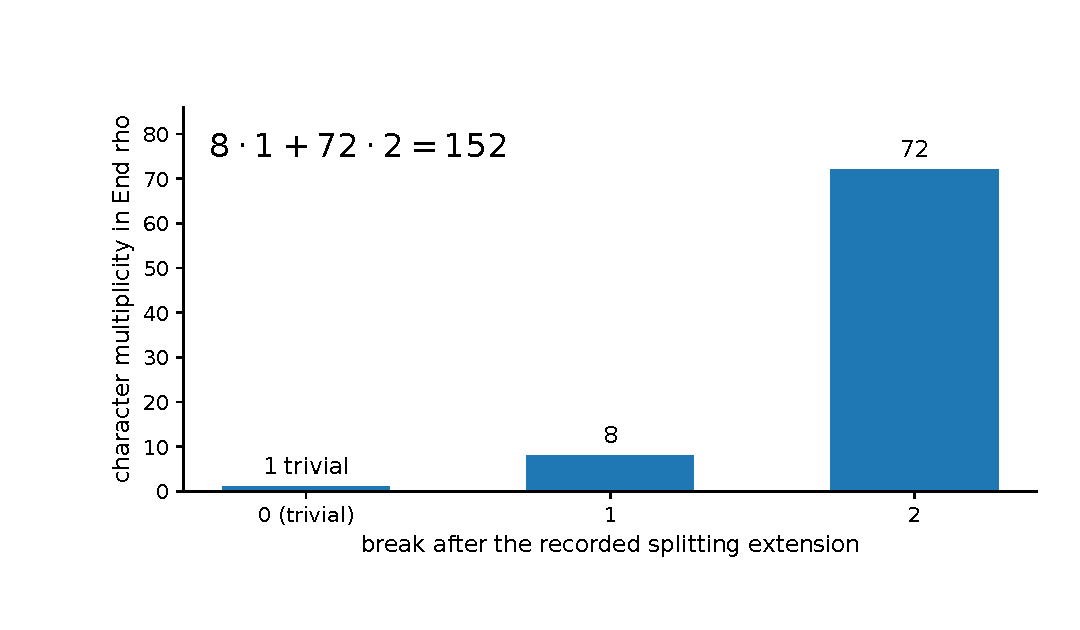
\includegraphics[width=\linewidth]{figures/V13.pdf}\end{center}
For the recorded source $\rho=A_1\otimes A_2$, each degree-three Heisenberg factor contributes one trivial conjugation character and eight nontrivial characters, at break one or two respectively. Under the original independence hypotheses, the tensor product contributes one trivial character, eight at break one, and seventy-two at break two.
\[
\operatorname{Sw}(\operatorname{End}\rho)=8+2\cdot72=152,
\qquad a(\operatorname{End}\rho)=81-1+152=232.
\]
The last subtraction uses wild irreducibility: the invariant endomorphisms are exactly the scalars. It does not require Frobenius to fix every individual character after the splitting extension.

The histogram is computed by enumerating the $9\times9$ pairs and taking the larger of the two unequal breaks. The arithmetic assertions that these are the source's genuine characters, that their breaks are as stated, and that the quotient factors are independent remain the inherited source hypotheses. Their role is exposed rather than replaced with a finite counting experiment.
\vfill\PlateSource{Exact character-count model}{Part III, Section 23.1}{59}
